% =============================================================================
%  A0 portrait poster (841 x 1189 mm) -- LUH / LUH|AI house style.
%  Compile with pdflatex (twice -- the header uses tikz "remember picture").
%  Figures expected in ./figures/:
%      task_memory_s17.png  model_architecture.png  compare_curves.pdf
%      logo_luh.jpg         logo_luhai.png          qr_repo.png
% =============================================================================
\documentclass[final]{article}

\usepackage[paperwidth=841mm,paperheight=1189mm,
            left=7mm,right=7mm,top=0mm,bottom=0mm]{geometry}
\usepackage[utf8]{inputenc}
\usepackage[T1]{fontenc}
\usepackage[table]{xcolor}
\usepackage{graphicx}
\usepackage{booktabs}
\usepackage{array}
\usepackage{amsmath,amssymb}
\usepackage{ragged2e}
\usepackage{enumitem}
\usepackage{tikz}
\usepackage[most]{tcolorbox}
\usepackage{textcomp}

% -- fonts: IBM Plex, as in the PowerPoint template; Helvetica if unavailable --
\IfFileExists{plex-sans.sty}{%
  \usepackage{plex-sans}%
  \IfFileExists{plex-mono.sty}{\usepackage{plex-mono}}{}%
}{%
  \usepackage[scaled]{helvet}%
}
\renewcommand{\familydefault}{\sfdefault}

\pagestyle{empty}
\frenchspacing                 % even word spacing, as in the PowerPoint version
\setlength{\parindent}{0pt}
\setlength{\fboxsep}{0pt}

% ------------------------------------------------------------------ colours --
\definecolor{luhblue}{HTML}{0B5394}
\definecolor{dark}{HTML}{202124}
\definecolor{mutedgrey}{HTML}{5F6368}
\definecolor{silver}{HTML}{9E9E9E}
\definecolor{panelgrey}{HTML}{8A8A8A}
\definecolor{tintblue}{HTML}{EEF3FA}
\definecolor{greybox}{HTML}{F3F3F3}
\definecolor{badgegrey}{HTML}{F3F3F3}
\definecolor{okgreen}{HTML}{137333}
\definecolor{nored}{HTML}{C5221F}
\definecolor{amber}{HTML}{B05A00}
\definecolor{hairline}{HTML}{D5D8DC}
\color{dark}

% -------------------------------------------------------------- type ladder --
\newcommand{\ptitle}{\fontsize{76}{88}\selectfont\bfseries}
\newcommand{\psubtitle}{\fontsize{52}{62}\selectfont\color{luhblue}}
\newcommand{\pauthor}{\fontsize{40}{50}\selectfont}
\newcommand{\plecture}{\fontsize{37}{46}\selectfont\color{silver}}
\newcommand{\psecfont}{\fontsize{46}{54}\selectfont\bfseries}
\newcommand{\pbody}{\fontsize{27}{35}\selectfont}
\newcommand{\pbodys}{\fontsize{26}{34}\selectfont}
\newcommand{\psmall}{\fontsize{25}{33}\selectfont}
\newcommand{\pcap}{\fontsize{22}{28}\selectfont\color{mutedgrey}}
\newcommand{\ptiny}{\fontsize{20}{26}\selectfont\color{mutedgrey}}
\newcommand{\phead}[1]{{\fontsize{34}{42}\selectfont\bfseries\color{luhblue}#1}\par\vspace{3mm}}

% ------------------------------------------------------------------ helpers --
% inline maths that shows up a lot
\newcommand{\Lw}{L}
\newcommand{\Lle}[1]{L\,\ensuremath{\leq}\,#1}
\newcommand{\Lge}[1]{L\,\ensuremath{\geq}\,#1}
\newcommand{\Leq}[1]{L\,=\,#1}
\newcommand{\tx}{\texttimes}
\newcommand{\pmm}{\textpm}
\newcommand{\mono}[1]{\texttt{#1}}

% numbered badge in a section title
\newcommand{\pbadge}[1]{%
  {\setlength{\fboxsep}{5mm}\colorbox{badgegrey}{%
   \makebox[10mm][c]{\textcolor{luhblue}{#1}}}}}

% numbered bullet for the key-insight list
\newcommand{\numdot}[1]{%
  \tikz[baseline=-0.9ex]\node[circle,fill=luhblue,text=white,inner sep=1.8mm,
        anchor=west,font=\fontsize{25}{25}\selectfont\bfseries] at (0,0) {#1};}

% one key insight: number, lead sentence, body
\newcommand{\insight}[3]{%
  \noindent\begin{minipage}[t]{15mm}\vspace{0pt}\numdot{#1}\end{minipage}%
  \begin{minipage}[t]{\dimexpr\linewidth-15mm\relax}\vspace{0pt}%
    \psmall\RaggedRight\textbf{#2} #3\end{minipage}\par}

% a panel: \begin{panel}{number}{title} ... \end{panel}
\newtcolorbox{panel}[2]{%
  enhanced, sharp corners, colback=white, colframe=panelgrey, boxrule=0.9pt,
  colbacktitle=luhblue, coltitle=white, titlerule=0mm,
  fonttitle=\psecfont, title={\pbadge{#1}\hspace{7mm}#2},
  left=11mm, right=11mm, top=9mm, bottom=9mm,
  toptitle=5mm, bottomtitle=5mm,
  before skip=0pt, after skip=0pt}

% a tinted callout inside a panel
\newtcolorbox{callout}[1][tintblue]{%
  sharp corners, colback=#1, colframe=#1, boxrule=0pt,
  left=7mm, right=7mm, top=6mm, bottom=6mm,
  before skip=0pt, after skip=0pt}

% ------------------------------------------------------------------ geometry --
\newlength{\lcolw}\setlength{\lcolw}{315mm}
\newlength{\rcolw}\setlength{\rcolw}{502mm}
\newlength{\colgap}\setlength{\colgap}{8mm}
\newlength{\colh}\setlength{\colh}{1006mm}

\begin{document}
\RaggedRight

% ============================================================ page furniture ==
\begin{tikzpicture}[remember picture,overlay]
  \begin{scope}[shift={(current page.north west)}]
    % the three LUH rules
    \fill[luhblue] (0mm,0mm)     rectangle (841mm,-7mm);
    \fill[luhblue] (0mm,-166mm)  rectangle (841mm,-173mm);
    \fill[luhblue] (0mm,-1182mm) rectangle (841mm,-1189mm);
    % logos, top right
    \node[anchor=north east,inner sep=0pt] at (836mm,-19mm)
      {
\includegraphics[height=59mm]{figures/logo_luh}};
    \node[anchor=north east,inner sep=0pt] at (626mm,-19mm)
      {
\includegraphics[height=59mm]{figures/logo_luhai}};
    % QR to the repository
    \node[anchor=north east,inner sep=0pt] at (836mm,-87mm)
      {
\includegraphics[width=58mm]{figures/qr_repo}};
    \node[anchor=north east,inner sep=0pt,align=right,text=mutedgrey,
          font=\fontsize{27}{34}\selectfont] at (770mm,-97mm)
      {Code, studies and\\winning checkpoints};
  \end{scope}
\end{tikzpicture}

% ==================================================================== header ==
\vspace*{24mm}
{\ptitle How Far Back Must the Gradient Reach?\par}
\vspace{7mm}
{\psubtitle Truncated BPTT length and memory in PPO on MiniGrid\par}
\vspace{10mm}
{\pauthor Anh Khoa Pham \quad\textperiodcentered\quad
 github.com/khoaphamanh/rl\_project\par}
\vspace{6mm}
{\plecture Poster presentation in context of the Reinforcement Learning
 lecture\par}

\vfill

% =================================================================== columns ==
\noindent
% ------------------------------------------------------------- LEFT COLUMN ---
\begin{minipage}[t][\colh][s]{\lcolw}%
\vspace*{0pt}% zero-height first item: both columns share a baseline

% ---------------------------------------------------------------- 1  TL;DR ---
\begin{panel}{1}{TL;DR}
  \pbody
  A recurrent policy can only use a memory that its \textbf{gradient} has
  taught it to write. One PPO pipeline, fixed; the only thing varied is how far
  back that gradient may reach --- the TBPTT window \Lw.
  \par\vspace{6mm}
  \textbf{The threshold is sharp.} \Lge{8} solves the task on every seed;
  \Lle{4} never beats a coin flip. Reaching further costs VRAM, not time.
  \par\vspace{10mm}

  \begin{tcbraster}[raster columns=4, raster column skip=5mm,
    raster equal height=rows, sharp corners, colback=tintblue,
    colframe=tintblue, boxrule=0pt, halign=center, valign=top,
    left=2mm, right=2mm, top=7mm, bottom=7mm]
    \begin{tcolorbox}
      {\fontsize{48}{54}\selectfont\bfseries\color{okgreen}1.000}\par
      \vspace{5mm}{\fontsize{21}{27}\selectfont\color{mutedgrey}
      success at\\ \Leq{8} and full BPTT}
    \end{tcolorbox}
    \begin{tcolorbox}
      {\fontsize{48}{54}\selectfont\bfseries\color{nored}0.500}\par
      \vspace{5mm}{\fontsize{21}{27}\selectfont\color{mutedgrey}
      success at \Leq{4}\\ (chance)}
    \end{tcolorbox}
    \begin{tcolorbox}
      {\fontsize{48}{54}\selectfont\bfseries\color{luhblue}8}\par
      \vspace{5mm}{\fontsize{21}{27}\selectfont\color{mutedgrey}
      steps of reach\\ suffice (4 do not)}
    \end{tcolorbox}
    \begin{tcolorbox}
      {\fontsize{48}{54}\selectfont\bfseries\color{luhblue}8\tx}\par
      \vspace{5mm}{\fontsize{21}{27}\selectfont\color{mutedgrey}
      the VRAM it costs\\ (the time: none)}
    \end{tcolorbox}
  \end{tcbraster}

  \vspace{7mm}
  {\fontsize{24}{31}\selectfont\color{mutedgrey}
   5 studies \tx{} 50 trials \tx{} 5 seeds = \textbf{250 training runs},
   \ensuremath{\approx}\,236 GPU-hours on one RTX 3060 Laptop (12\,GB).\par}
\end{panel}

\vfill

% ------------------------------------------------------------- 3  Approach ---
\begin{panel}{3}{Approach}
  \phead{Network}
  \centering
  
\includegraphics[width=245mm]{figures/model_architecture}
  \par\vspace{2mm}
  \RaggedRight
  {\pcap 7\,\tx\,7\,\tx\,3 view \textrightarrow{} one-hot (980) \textrightarrow{}
   encoder \textrightarrow{} linear actor + linear critic. The encoder is the
   \textbf{only} difference between arms: an MLP (memoryless) or a single GRU
   layer carrying \mono{h} forward.\par}
  \vspace{9mm}

  \phead{The knob under study}
  {\pbodys Before every update the rollout is cut at each \textbf{episode
   boundary and every \Lw{} steps}. A chunk starting mid-episode is seeded with
   the hidden state the rollout recorded there, so the forward pass still sees
   the whole episode and \textbf{only the backward pass is shortened} --- every
   GRU arm carries identical information forward.\par}
  \vspace{8mm}

  \begin{callout}[greybox]
    {\fontsize{25}{32}\selectfont\bfseries One PPO iteration\par}
    \vspace{4mm}
    {\fontsize{22}{29}\selectfont
     1\; collect W\,=\,32 workers \tx{} T\,=\,361 steps, recording
        (o, a, log\,\ensuremath{\pi}, V, r, d, \textbf{h})\par
     \vspace{1.5mm}
     2\; GAE over the \textbf{whole} rollout, before any split;
        standardise $\hat{A}$\par
     \vspace{1.5mm}
     \textcolor{amber}{3\; \textbf{cut into chunks of \ensuremath{\leq}\,L
        steps, each seeded with its stored h}}\par
     \vspace{1.5mm}
     4\; 3 shuffled epochs of the clipped PPO loss; padding never enters it\par}
    \vspace{4mm}
    {\fontsize{21}{27}\selectfont\color{mutedgrey}
     L\,=\,\ensuremath{\infty} (full BPTT) cuts at episode boundaries only; a
     smaller L means more, shorter sequences --- $\lceil T/L \rceil$ of them.\par}
  \end{callout}
  \vspace{9mm}

  \phead{Tuning protocol}
  {\pbodys
   \begin{itemize}[leftmargin=9mm,itemsep=4mm,topsep=4mm,parsep=0pt]
     \item One Optuna study \textbf{per arm}: 50 TPE trials over
           \textbf{identical} ranges --- no arm is judged on another's settings.
     \item Each trial trains the same 5 seeds for 1000 iterations and is scored
           \textbf{mean \textminus{} std across seeds} on 50 held-out mazes.
     \item Nothing that buys compute is searchable; the minibatch size is set
           by a VRAM probe, so every arm is measured at the \textbf{same memory
           budget}.
   \end{itemize}\par}
\end{panel}

\vfill

% -------------------------------------------- 6  Limitations & future work ---
\begin{panel}{6}{Limitations \& Future Work}
  {\pbodys
   \textbf{One task, one architecture, one algorithm.} L \ensuremath{\in}
   \{5,\,6,\,7\} was never run, so the threshold is \textbf{bracketed, not located}, and five
   seeds separate 0.5 from 1.0 safely but support no finer claim.
   \begin{itemize}[leftmargin=9mm,itemsep=4mm,topsep=5mm,parsep=0pt]
     \item \textbf{Locate the threshold.} Sweep L \ensuremath{\in}
           \{5,\,6,\,7\} and set the
           corridor length directly instead of leaving it to the environment
           --- a causal test of the gap account.
     \item \textbf{Add R2D2-style burn-in.} Does a short window then behave
           like a long one? If so the threshold is about optimisation, not the
           gradient path.
     \item \textbf{Repeat with an LSTM and a small transformer}, where the
           analogous knob is the attention window.
   \end{itemize}\par}
  \vspace{7mm}
  {\color{hairline}\rule{\linewidth}{0.8mm}}
  \vspace{4mm}
  {\ptiny \textbf{References.} Hausknecht \& Stone 2015 \textperiodcentered{}
   Kapturowski et al.\ 2019 (R2D2) \textperiodcentered{} Ni et al.\ 2022
   \textperiodcentered{} Schulman et al.\ 2017 (PPO) \textperiodcentered{}
   Chevalier-Boisvert et al.\ 2023 (MiniGrid)\par}
\end{panel}

\end{minipage}%
\hspace{\colgap}%
% ------------------------------------------------------------ RIGHT COLUMN ---
\begin{minipage}[t][\colh][s]{\rcolw}%
\vspace*{0pt}% zero-height first item: both columns share a baseline

% ------------------------------------------ 2  Motivation & problem setting ---
\begin{panel}{2}{Motivation \& Problem Setting}
  \pbody
  In a POMDP the optimal action depends on information that has left the
  observation. The usual remedy is a recurrent policy; the usual concession is
  to \textbf{truncate the backward pass to \Lw{} steps}, a value inherited in
  silence from whatever codebase one starts from.
  \par\vspace{5mm}
  \mono{MiniGrid-MemoryS17Random-v0} makes it measurable. A cue visible only in
  the west room decides which prong of the T-junction at the far end pays, and
  the 7\,\tx\,7 egocentric view makes both prongs identical: a
  \textbf{memoryless policy is capped at 0.5}, so the gap from 0.5 to 1.0 is
  exactly the memory a run has acquired.
  \par\vspace{8mm}

  \begin{callout}
    {\psmall\color{luhblue}
     \textbf{Q1} --- How far back must the gradient reach? Carrying \mono{h}
     forward is free at any \Lw, so is a short window enough to \textbf{learn
     what to store}?\par
     \vspace{4mm}
     \textbf{Q2} --- What does that reach cost in time and in VRAM? A shorter
     window is intuitively cheaper --- we check whether it is.\par}
  \end{callout}
  \vspace{9mm}

  \centering
  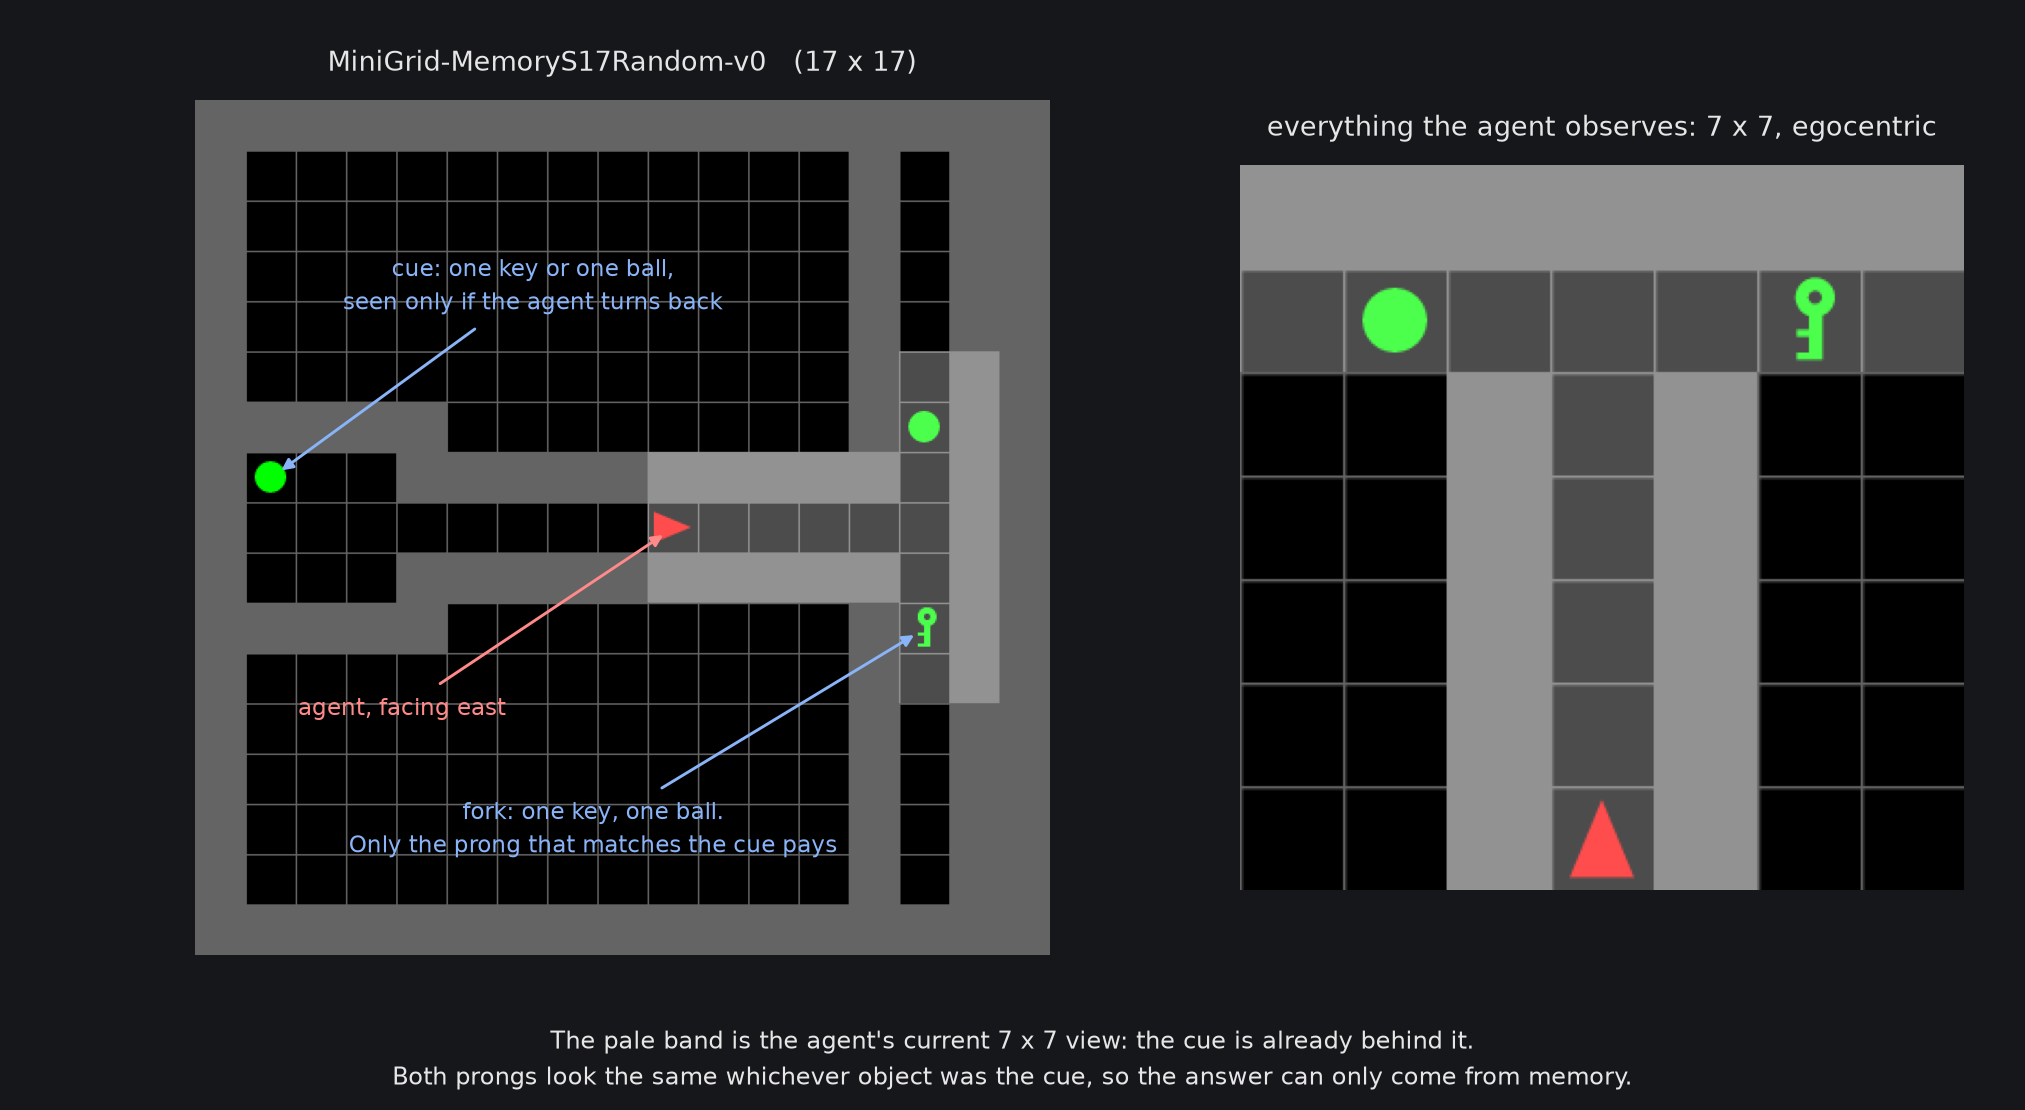
\includegraphics[width=320mm]{figures/task_memory_s17}
\end{panel}

\vfill

% -------------------------------------------------------------- 4  Results ---
\begin{panel}{4}{Results}
  \psmall
  \setlength{\tabcolsep}{0pt}
  \setlength{\heavyrulewidth}{1.1mm}
  \setlength{\lightrulewidth}{0.5mm}
  \renewcommand{\arraystretch}{1.55}
  \begin{tabular}{@{}p{126mm}>{\centering\arraybackslash}p{87mm}%
                   >{\centering\arraybackslash}p{87mm}%
                   >{\centering\arraybackslash}p{58mm}%
                   >{\centering\arraybackslash}p{69mm}%
                   >{\centering\arraybackslash}p{53mm}@{}}
    \arrayrulecolor{luhblue}\toprule
    \textbf{\textcolor{luhblue}{arm}} &
    \textbf{\textcolor{luhblue}{return}} &
    \textbf{\textcolor{luhblue}{success rate}} &
    \textbf{\textcolor{luhblue}{steps}} &
    \textbf{\textcolor{luhblue}{minibatch}} &
    \textbf{\textcolor{luhblue}{time}} \\
    \midrule
    MLP (memoryless) & 0.556\,\pmm\,0.029 & 0.592\,\pmm\,0.027 & 24.3 & 1024 & 1.3\,h \\
    GRU, \Leq{1}     & 0.573\,\pmm\,0.064 & 0.588\,\pmm\,0.068 &  9.8 & 4096 & 2.6\,h \\
    GRU, \Leq{4}     & 0.492\,\pmm\,0.001 & 0.500\,\pmm\,0.000 &  7.0 & 4096 & 1.6\,h \\
    \rowcolor{tintblue}
    GRU, \Leq{8}     & \textcolor{okgreen}{\textbf{0.958\,\pmm\,0.004}}
                     & \textcolor{okgreen}{\textbf{1.000\,\pmm\,0.000}}
                     & 16.8 & 4096 & 2.0\,h \\
    \rowcolor{tintblue}
    GRU, full BPTT   & \textcolor{okgreen}{\textbf{0.958\,\pmm\,0.002}}
                     & \textcolor{okgreen}{\textbf{1.000\,\pmm\,0.000}}
                     & 16.8 &  512 & \textcolor{okgreen}{\textbf{1.3\,h}} \\
    \bottomrule
  \end{tabular}
  \par\vspace{4mm}
  {\pcap Winning trial per study, averaged over its five seeds; \pmm{} is the
   spread across seeds. No setting produced an intermediate score.\par}
  \vspace{9mm}

  \centering
  
\includegraphics[width=360mm]{figures/compare_curves}
  \par\vspace{3mm}
  \RaggedRight
  {\pcap Mean over 5 seeds, band at \pmm\,1 std, dashed line at chance. The two
   solving arms separate before iteration 400; the three failing arms never
   leave the chance line.\par}
\end{panel}

\vfill

% --------------------------------------------------------- 5  Key insights ---
\begin{panel}{5}{Key Insights}
  \insight{1}{Carrying \mono{h} forward is not what matters.}{Every GRU arm
    does it identically, including the ones that fail. What separates them is
    whether the \textbf{gradient} reaches back to the observation that filled
    \mono{h} --- and reaching past 8 adds nothing.}
  \vspace{7mm}

  \insight{2}{What has to fit inside \Lw{} is the \textbf{gap}, not the
    episode.}{The gap is the number of actions between the agent's last
    sighting of the cue and its choice at the fork. By BFS over the
    environment's own visibility model, a gap \ensuremath{\leq}\,8 is
    attainable in \textbf{62\,\%} of mazes but a gap \ensuremath{\leq}\,4 in
    only \textbf{26\,\%};
    replaying the checkpoints, cue and decision share a chunk in 16\,\% of the
    \Leq{8} agent's episodes and in \textbf{0 of 50} of the \Leq{4} agent's.}
  \vspace{7mm}

  \insight{3}{The failing arms are not partially remembering.}{At 7.0 steps
    the \Leq{4} arm dashes straight to the fork and always picks the same side
    --- exactly 25/50 here. Its across-seed std of 0.000 is \textbf{arithmetic,
    not convergence}.}
  \vspace{7mm}

  \insight{4}{The reach costs memory, not time.}{Full BPTT is the
    \textbf{fastest} GRU arm (1.3\,h vs 2.6\,h at \Leq{1}) and the earliest
    (0.95 success at a median of 370 iterations vs 640 for \Leq{8}): halving
    \Lw{} doubles the padded, launch-bound sequences. What it pays is VRAM ---
    minibatch 512 vs 4096.}
  \vspace{10mm}

  \begin{callout}
    {\pbodys\color{luhblue}\textbf{Recommendation.} On this task: full BPTT,
     with \Leq{8} as the fallback on a smaller GPU. Below 8 you do not get a
     cheaper solution --- you get the MLP's guessing policy at GRU prices.\par}
  \end{callout}
\end{panel}

\end{minipage}

\vspace*{7mm}
\end{document}
